The focus of this Section is the coupled effects of \gls{He} implantation and hydrogen transport.
To this end, the experiment of Ialovega and co-workers \sidecite{ialovega_hydrogen_2020} is reproduced with the \gls{He} bubble model described in this Chapter coupled to \gls{festim}.

\subsection{Experiment}

A \SI{100}{\micro\metre} thick tungsten sample was pre-damaged with \SI{75}{eV} He at \SI{1073}{K}.
The \gls{He} flux was \SI{2.3e22}{m^{-2}.s^{-1}} and the exposure time was \SI{13}{s}.
An initial cleaning \gls{tds} was performed up to \SI{870}{K}.

Sequential deuterium loading and \gls{tds} were then repeated five times.
\SI{250}{eV} deuterium were implanted at room temperature with a flux of \SI{1.7e16}{m^{-2}.s^{-1}} and a \gls{fluence} of \SI{4.5e19}{m^{-2}}.
The \gls{tds} phase ramps up to \SI{1350}{K} (\SI{1250}{K} for the first \gls{tds}) at a rate of \SI{1}{K.s^{-1}}.

\subsection{Bubble growth simulation}
The quantities $c_b$ and $\langle r_b \rangle$ have been computed from the helium bubble model described in \refsec{helium model description} (see \reffig{trap bubbles distribution}).
The helium implantation distritbuion is a Gaussian with a mean value of \SI{1.5}{nm} and a standard deviation of \SI{0.8}{nm} corresponding to a \SI{75}{eV} He exposure calculated with \gls{srim}. 
The other parameters are unchanged.

\subsection{\gls{festim} simulation}
Four traps are simulated with \gls{festim}: traps 1-3 are pre-existing defects and trap 4 represents the traps induced by \gls{He} bubbles.
The detrapping energies and trap densities are set as free parameters, including the trap density $n_b$ (see \reftab{trap properties}).

Considering deuterium is trapped on the surface of \gls{He} bubbles, the bubble trap density $n_b$ is given by:

\begin{equation}
    n_b = f \cdot c_b \cdot \Ab(\langle r_b \rangle)
\end{equation}
where $f$ is a free parameter representing the number of trapping site per unit surface, $\Ab = 4\pi \langle r_b \rangle^2$ is the area in \si{m^2} of a spherical bubble of radius $\langle r_b \rangle$, and $c_b$ is the concentration of bubbles in $\si{m^{-3}}$.


\begin{figure}[h!]
    \centering
    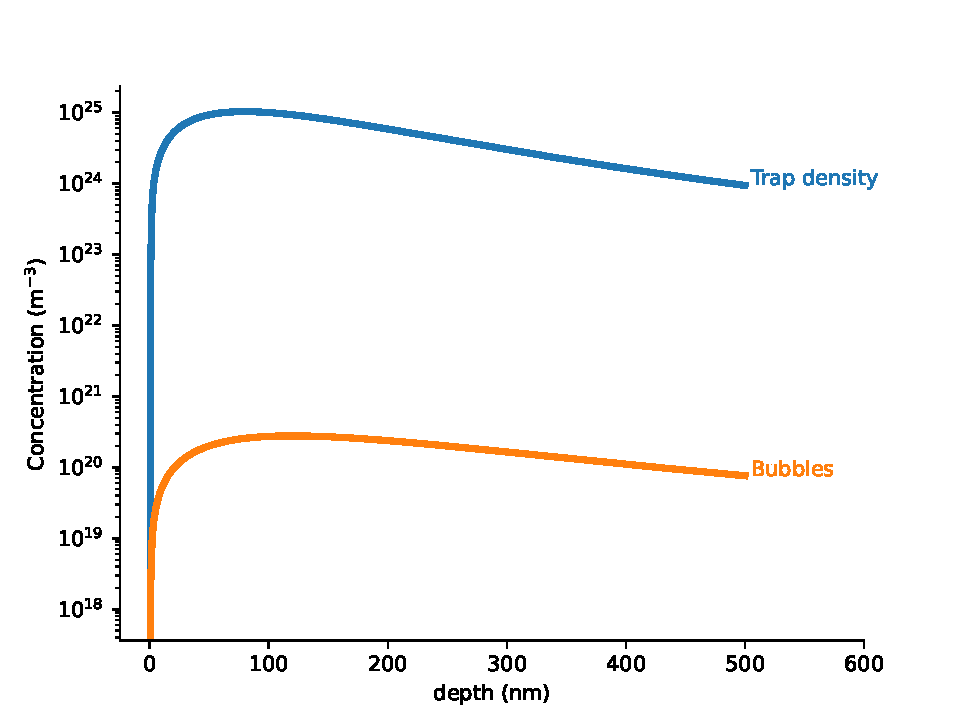
\includegraphics[width=\linewidth]{Figures/Chapter5/trap_bubble_distribution.pdf}
    \caption{Spatial distribution of the bubbles density and the equivalent trap density (assuming $f=\SI{3e18}{m^{-2}}$).}
    \labfig{trap bubbles distribution}
\end{figure}


\begin{table}[!h]
    \caption{Trap properties used to fit the \gls{tds} spectra. The density distribution $n_b$ as well as detrapping energies $E_p$ are assumed constant across TDS experiments.}
    \begin{tabular}{r l l l l l}
    \\
     & $k_0$ & $E_k$ & $p_0$ & $E_p$ & $n$ \\
     \ & [\si{m^{3}.s{-1}}] & [\si{eV}] & [\si{s^{-1}}] & [\si{eV}] & [\si{m^{-3}}] \\
    \\
    Trap 1 & \multirow{7}{*} { $9 \times 10 ^{-17}$ } & \multirow{7}{*} { 0.39 } & \multirow{7}{*} { $10^{13}$ } & free & free \\
    \\
    Trap 2 & & & & free & free \\
    \\
    Trap 3 & & & & free & free \\
    \\
    Trap bubbles & & & & free & $n_b$ \\
    \end{tabular}
    \labtab{trap properties}
\end{table}

The diffusion coefficient of deuterium (\si{m^2.s^{-1}}) was set to $4.1\times 10 ^{-7} \exp{(-0.39/k_B T)}$ \sidecite{frauenfelder_solution_1969}.
The \SI{250}{eV} deuterium implantation was represented by a Gaussian distribution with a mean implantation depth \SI{10}{nm} and a standard deviation of \SI{4.5}{nm} (calculated from \gls{srim} \sidecite{ziegler_srim_2010}).
Finally, an instantaneous recombination was assumed on the surfaces.

Using the parametric optimisation method presented in \refsec{methodology}, the free parameters are identified.

\subsection{Results}

The properties obtained by the fitting procedure (see \reftab{trap properties results}) fitted well the three \gls{tds} spectra (see \reffig{fitted TDS}).
As explained in \cite{ialovega_hydrogen_2020}, the last bump of desorption (around \SI{600}{K}) is due to a temperature control issue and was therefore ignored in the fitting procedure.
The detrapping energies of traps 1, 2 and 3 were found to be \SI{1.08}{eV}, \SI{1.20}{eV} and \SI{1.38}{eV} respectively, whereas the trap attributed to \gls{He} bubbles has a detrapping energy of \SI{1.45}{eV}.


\begin{table}[!h]
    \caption{Results of the fitting procedure. Detrapping energies $E_p$ are given in \si{eV}, trap densities in \si{at.fr.} and $f$ in \si{m^{-2}}.}
    \begin{tabular}{r l l l l l l l l}
    \\
    &\multicolumn{2}{l}{Trap 1}  & \multicolumn{2}{l}{Trap 2} & \multicolumn{2}{l}{Trap 3} &\multicolumn{2}{l}{Trap bubbles} \\
     & $E_p$ & $n$ ($\times 10 ^{-3}$) & $E_p$ & $n$ ($\times 10 ^{-3}$) & $E_p$ & $n$ ($\times 10 ^{-3}$) & $E_p$ & $f$ ($\times 10 ^{18}$) \\
    \\
    1st \gls{tds} & - & 0.00 & - & 0.00 & - & 0.00 & 1.42 & $3.00$ \\
    \\
    2nd \gls{tds} & 1.08 & $2.20$ & 1.20 & $1.80$ & 1.37 & $2.00$ & 1.42 & $3.00$ \\
    \\
    5th \gls{tds} & 1.08 & $3.38$ & 1.20 & $3.10$ & 1.37 & $1.50$ & 1.42 & $3.00$ \\
    \end{tabular}
    \labtab{trap properties results}
\end{table}

This would mean that if the \gls{tds} were run up to temperature around \SI{1600}{K}, $\mathrm{He}_1\mathrm{V}_1$ clusters could dissociate resulting in additional free trapping sites for \gls{H} and therefore different \gls{tds} spectra.

The \gls{H} retention is not dominated by \gls{He}-bubbles trapping but rather by pre-existing defects.

\begin{figure}[h!]
    \centering
    \begin{subfigure}{\linewidth}
        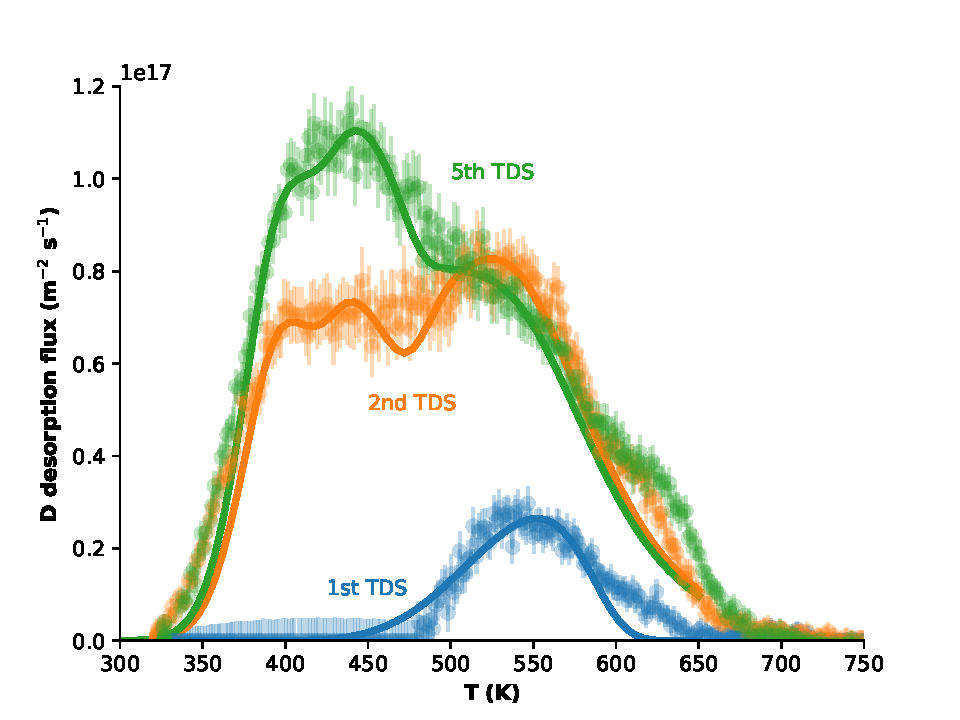
\includegraphics[width=\linewidth]{Figures/Chapter5/ialovega_tds.pdf}
        \caption{Experimental TDS spectra fitted with FESTIM. Experimental points are taken from \cite{ialovega_hydrogen_2020}.}
        \labfig{3 TDS}
    \end{subfigure}
    \begin{subfigure}{\linewidth}
        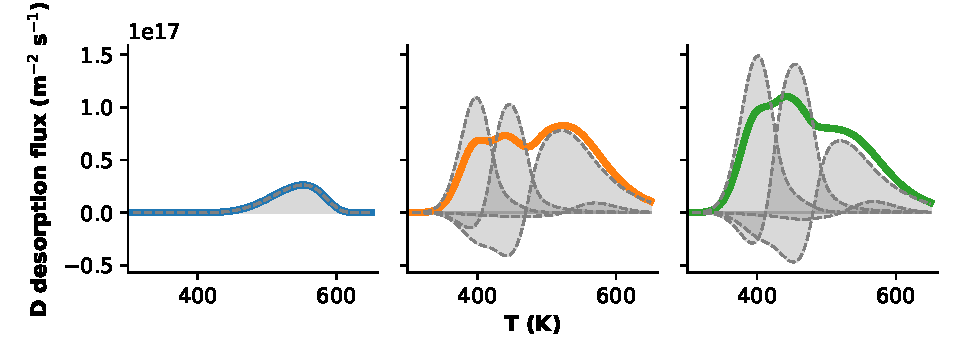
\includegraphics[width=\linewidth]{Figures/Chapter5/tds_trap_distribution.pdf}
        \caption{Traps contribution to the TDS spectra.}
        \labfig{trap contributions}
    \end{subfigure}
    \caption{Results of the TDS fitting procedure.}
    \labfig{fitted TDS}
\end{figure}

\begin{figure}
    \centering
    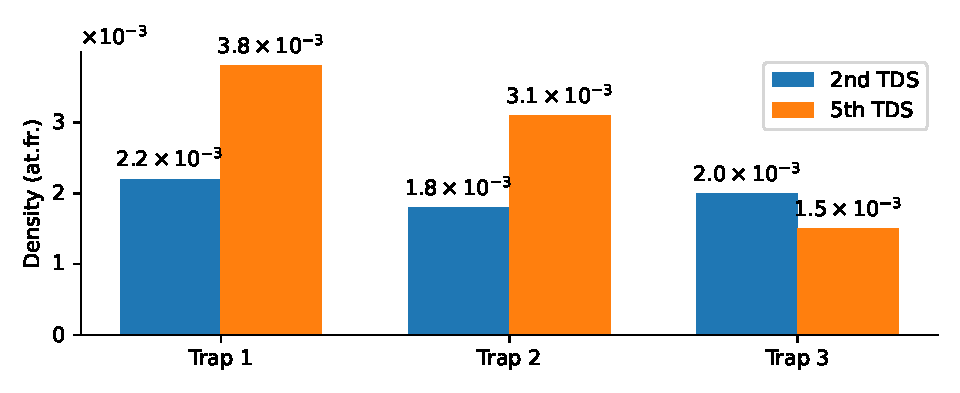
\includegraphics[width=\linewidth]{Figures/Chapter5/trap_densities.pdf}
    \caption{Evolution of the trap densities between the second and fifth TDS.}
    \labfig{density evolution}
\end{figure}

The densities of traps 1 and 2 increased from the 2nd to the 5th \gls{tds} (see \reffig{density evolution}).
However, the density of trap 3 decreased slightly (which is also visible on the \gls{tds} spectra shown in \reffig{fitted TDS}).
The processes at stake cannot yet be precisely described. 

One possible interpretation of the results is:
\begin{itemize}
    \item Initial state: the sample has some pre-existing defects %(proof from PAS that there are pre-existing defects before He implantation)
    \item \gls{He} implantation: all pre-existing defects are saturated with \gls{He} and bubbles are formed
    \item 1st \gls{D} implantation: \gls{D} can only be trapped around bubbles since defects are saturated with \gls{He}
    \item 1st \gls{tds} (up to \SI{1250}{K}): \gls{D} is detrapped from bubbles is desorbed (\SI{550}{K} peak), \gls{He} dissociates from pre-existing defects 
    \item 2nd \gls{D} implantation: \gls{D} is trapped around bubbles and in the non-saturated defects
    \item 2nd \gls{tds} (up to \SI{1350}{K}): \gls{D} is detrapped from bubbles is desorbed (\SI{550}{K} peak) and from non-saturated defects (peaks 400K, 450K and 500K) + \gls{He} trapped in deeper traps dissociate (because the \gls{tds} goes to higher temperatures)
    \item 3rd to 5th \gls{D} implantations: \gls{D} is trapped around bubbles and in pre-existing defects
    \item 3rd to 5th \gls{tds}: \gls{D} is detrapped from bubbles and pre-existing defects (now more available than at the 2nd \gls{tds})
\end{itemize}
This interpretation is represented (in a simplified way) on \reffig{ialovega experiment interpretation}.


\begin{figure*}
    \centering
    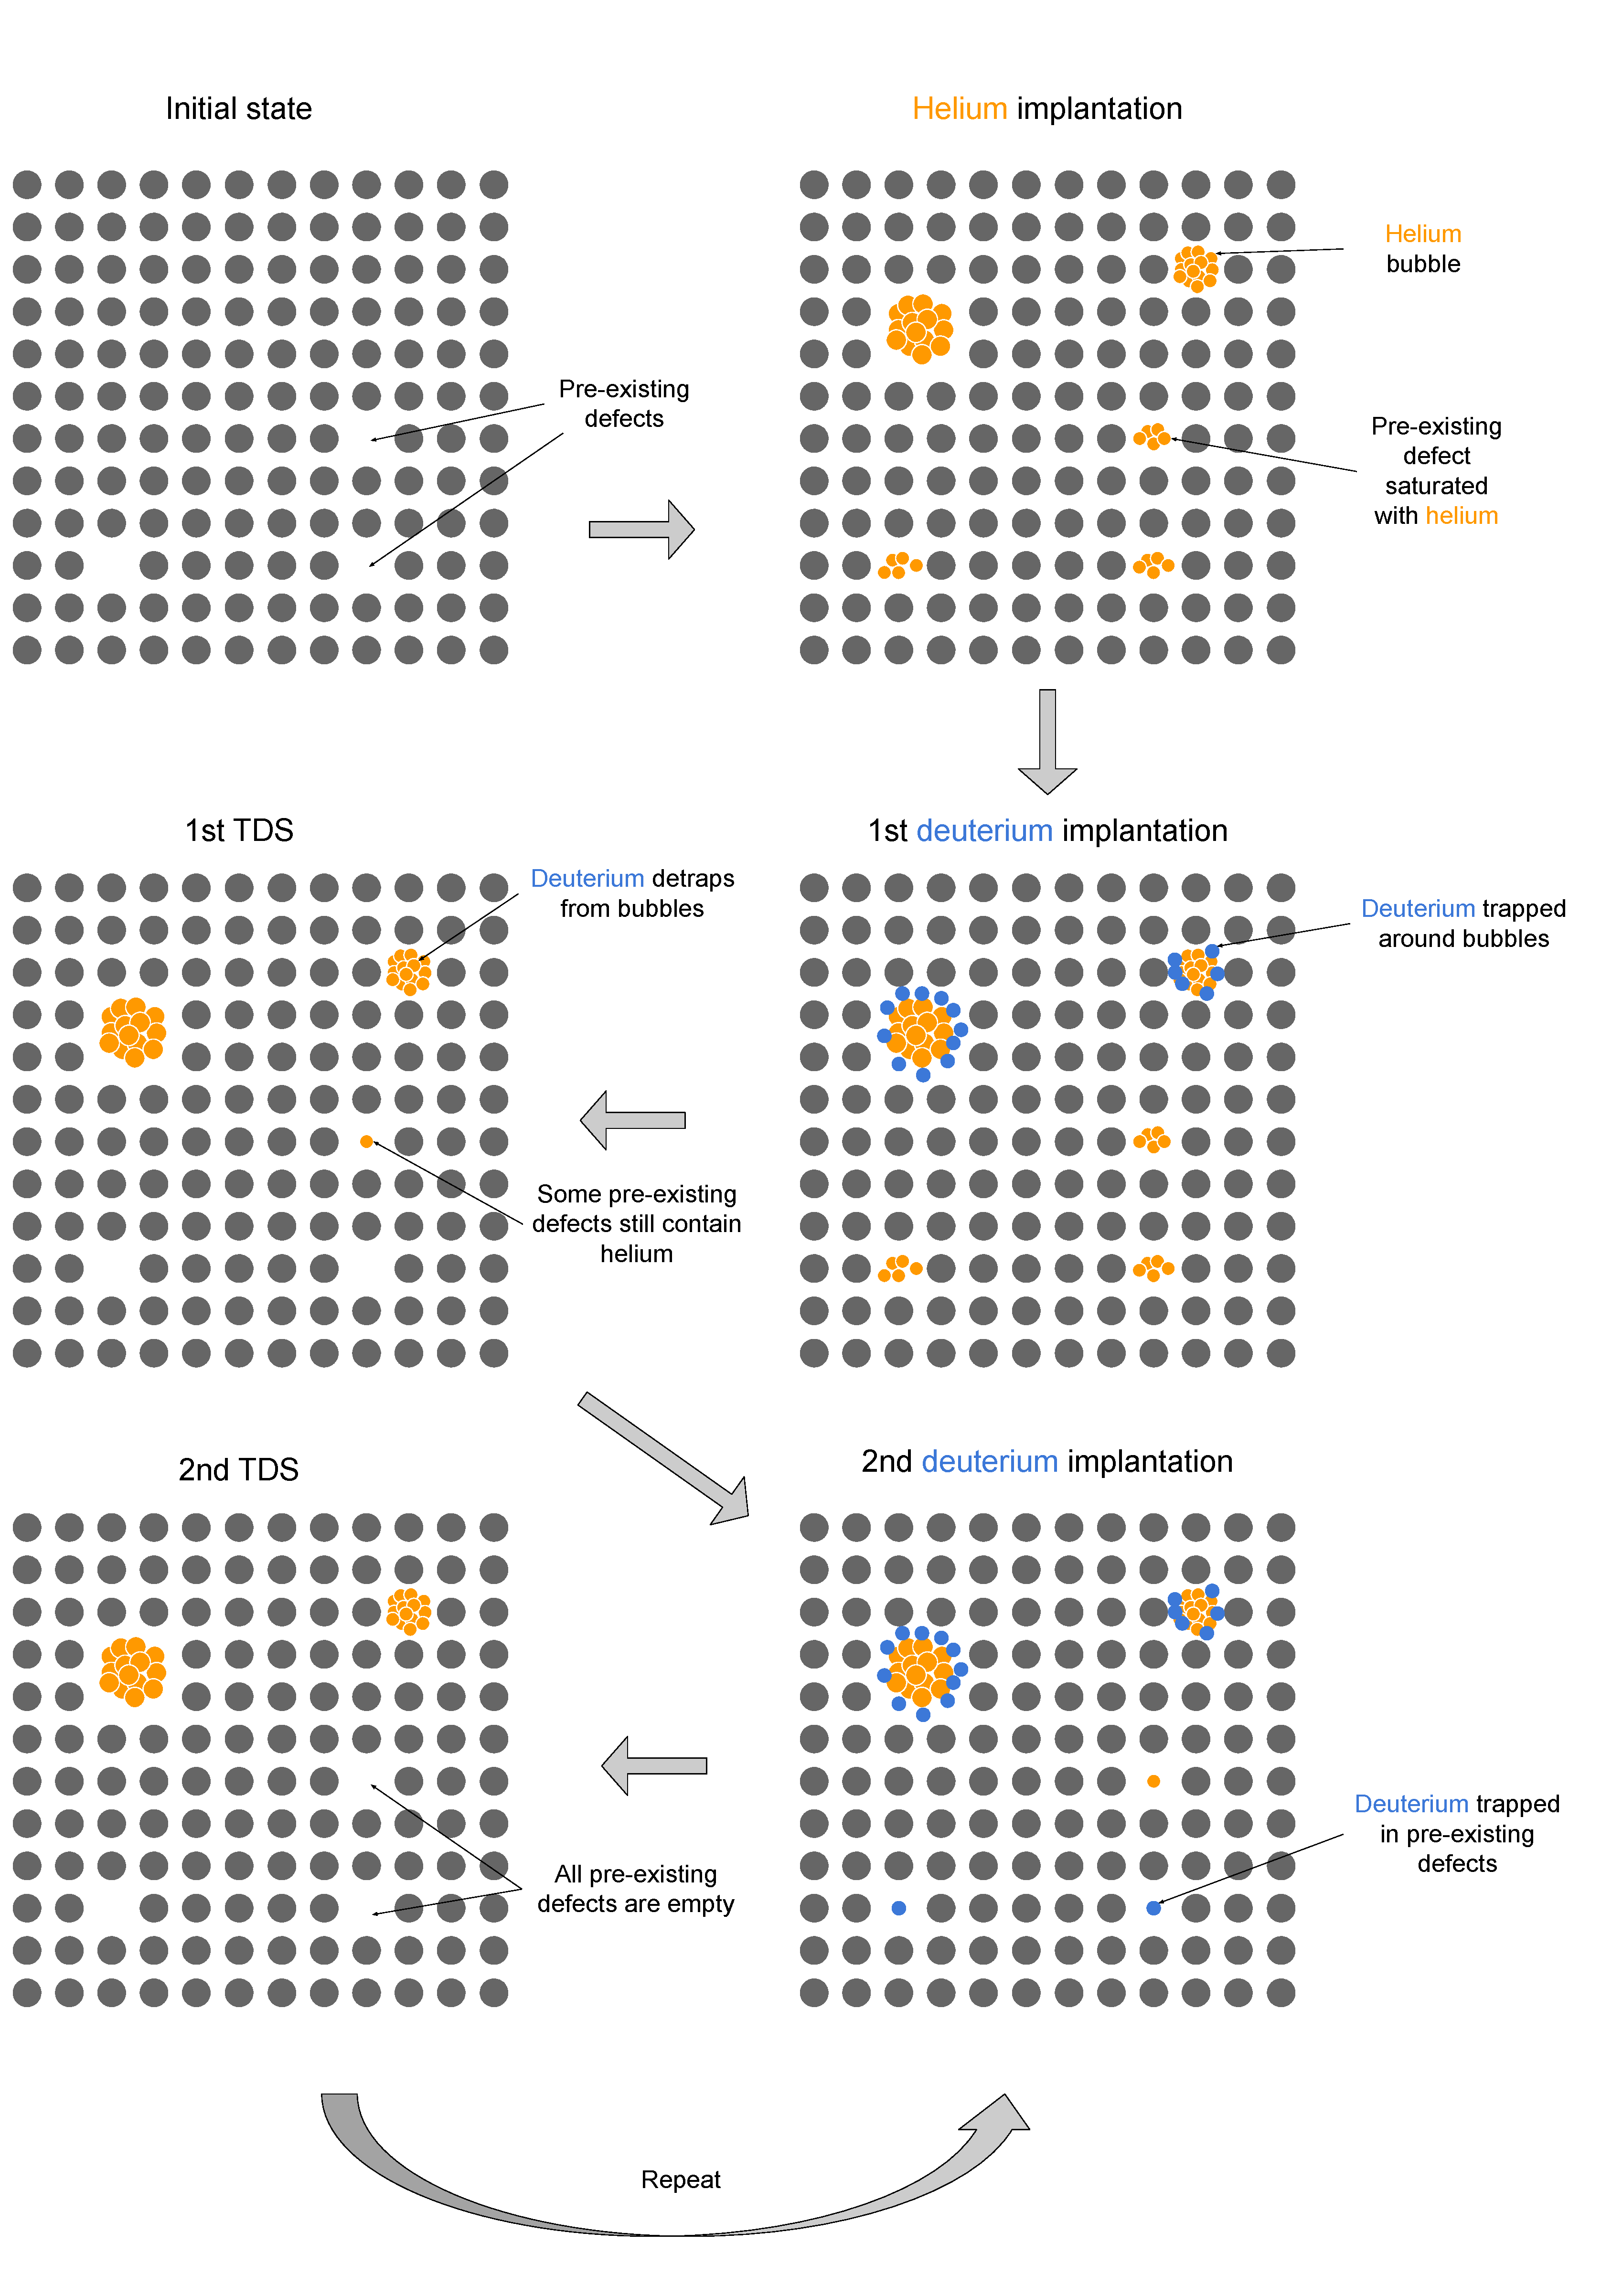
\includegraphics[width=\linewidth]{Figures/Chapter5/sketch ialovega experiment.pdf}
    \caption{Schematic interpretation of the simulation results showing the several stages of the experiment (from \gls{He} implantation to TDS cycles).}
    \labfig{ialovega experiment interpretation}
\end{figure*}
